\documentclass[preprint, floatfix, pra, showpacs, showkeys]{revtex4}
\usepackage{graphicx}
\usepackage{dcolumn}

\newcommand{\threej}[6]{\ensuremath{\left({#1\atop #4}{#2\atop #5}
{#3\atop #6}\right)}}
\newcommand{\sixj}[6]{\ensuremath{\left\{{#1\atop #4}{#2\atop #5}
{#3\atop #6}\right\}}}

\begin{document}

\title{The Flexible Atomic Code: I. Atomic Structure} 
\author{Ming Feng Gu}
\affiliation{Center for Space Research, Massachusetts Institute of Technology,
Cambridge, MA 02139} 
\email[Email: ]{mfgu@space.mit.edu}

\begin{abstract}
In this and subsequent papers, we describe a complete software package for
the computation of various atomic data, such as energy levels,
radiative transition, collisional excitation and ionization by electron impact,
photoionization, autoionization, and their inverse processes radiative
recombination and dielectronic capture. 
This paper deals with the atomic structure part
and the calculation of radiative transition rates. The bound states of the
atomic system are calculated in the configuration mixing approximation with
convenient specification of mixing schemes. The radial orbitals for the
construction of basis states are derived from a modified self-consistent
Dirac-Fock-Slater 
iteration on a fictitious mean configuration with fractional occupation
numbers, representing the average electron cloud of the configurations
included in the calculation. The radiative transition rates are calculated in
the single multipole approximation with arbitrary ranks.
\end{abstract}

\pacs{31.15.-p, 32.70.Cs}
\keywords{Atomic structure; Radiative transition}

\maketitle

\section{Introduction}
This is the first of a series of papers introducing a complete software
package, the Flexible Atomic Code (FAC), for the computation of various atomic
radiative and collisional processes. A fully relativistic approach based on
the Dirac equation is used throughout the entire package which allows its
application to ions with large values of nuclear charge. Currently, FAC
is able to treat radiative transition, direct collisional excitation and
ionization by electron impact, non-resonant photoionization and radiative
recombination, autoionization and dielectronic recombination. These processes
are essential for the interpretation of laboratory and astrophysical 
spectroscopic data. The main goal of creating such a comprehensive package is
to integrate various atomic processes within a single theoretical framework,
ensure the self-consistency between different parts, and provide a uniform,
flexible and easy-to-use user interface for accessing all computational tasks. 

Many computer programs now exist for the calculation of atomic processes,
using either non-relativistic approximations (some including relativistic
effects through the Breit-Pauli Hamiltonian) or fully relativistic
methods. Most of them are mainly concerned with the atomic structure part and
bound-bound processes, e.g., the non-relativistic configuration interaction
codes CIV3 \cite{hibbert75} and SUPERSTRUCTURE \cite{eissner74}, the widely
used program of \textcite{cowan81}, the multi-configuration Hartree-Fock (MCHF)
program of \textcite{fischer00}, and the multi-configuration Dirac-Fock (MCDF)
code of \textcite{grant80}. Many newer programs for continuum processes make
use of the output from these structure codes for bound state wave
functions. This sometimes leads to 
a different treatment of continuum states from that of bound states. More
importantly, the communication between different programs tends to complicate
the user interface, and makes it difficult for people other than the authors
of the codes to efficiently use them. 

There also exist several integrated
packages for the calculation of a variety of atomic processes, e.g., the ATOM
package \cite{amusia97}, the HULLAC package \cite{barshalom01}, and the fully
relativistic code (SZ) developed by \textcite{sampson89} and
\textcite{zhang89}. These programs treat continuum as well as bound
processes. In  
ATOM, the radial wave functions for bound and continuum orbitals are obtained
using the self-consistent field Hartree-Fock method or the frozen-core
Hartree-Fock method. A relativistic version based on the Dirac equation is
also available. Such a procedure tends to be very time consuming, especially
for continuum processes, where the number of continuum orbitals needed is
large. The HULLAC package and SZ are both based on the Dirac equation, and use
a single, local, central potential for the solution of radial orbitals. This
approach is very efficient because the orthogonality of 
different orbitals is automatically ensured. Both codes use the distorted wave
(DW) approximation for continuum processes. The difference between them is
mainly in the way the local central potential is obtained. In HULLAC, 
a parametric potential is used and the parameters in the potential are derived
by minimizing the average energies of some selected configurations
\cite{klapisch77}. In SZ, one 
constructs a fictitious mean configuration with fractional occupation numbers
that takes into account the electron screening of all configurations involved
in the physical processes to be calculated. A self-consistent
Dirac-Fock-Slater iteration is then 
performed on this mean configuration to derive the local central potential. 
Although various results from these two codes have been published over the
years, the programs are not available to the general public. The present
package combines the strengths of these existing atomic codes, with
modifications to numerical procedures made to extend the capability and
improve the efficiency and robustness. The entire package is publicly
available upon request to the author.

This paper presents the theoretical background related
to the atomic structure calculation and bound-bound processes, and
compares the results with previous publications. In
Section \ref{sec_theory}, we outline the theory, and discuss the key numerical
techniques used in the program. Section \ref{sec_results} presents a detailed
comparison between the results obtained with this package and those of
existing codes. A brief summary is given in Section \ref{sec_conclusions}.

\section{Theory and Numerical Techniques}
\label{sec_theory}
The energy levels of an atomic ion with $N$ electrons are obtained by
diagonalizing the relativistic Hamiltonian $H$. In atomic units, which we shall
use throughout the papers, it reads
\begin{equation}
\label{eq_hamilton}
H = \sum_{i=1}^{N} H_{D}(i) + \sum_{i<j}^{N}\frac{1}{r_{ij}},
\end{equation}
where $H_{D}(i)$ is the single-electron Dirac Hamiltonian for the potential
due to the nuclear charge. The basis states $\Phi_{\nu}$, which are usually
referred to as configuration state functions (CSF), are antisymmetric sums of
products of $N$ one-electron Dirac spinors $\varphi_{n\kappa m}$
\begin{equation}
\label{eq_spinor}
\varphi_{n\kappa m} = \frac{1}{r}\left(\begin{array}{c}
P_{n\kappa}(r) \chi_{\kappa m}(\theta, \phi, \sigma)\\
iQ_{n\kappa}(r) \chi_{-\kappa m}(\theta, \phi, \sigma)
\end{array}\right),
\end{equation}
where $\chi_{\kappa m}$ is the usual spin-angular function. $n$ is the
principal quantum number, $\kappa$ is the relativistic angular quantum number
, which is related to the orbital and total angular momentum through
\begin{equation}
\kappa = (l-j)(2j+1),
\end{equation}
and $m$ is the $z$-component of the total angular momentum $\mathbf{j}$. In
coupling the angular momenta of successive shells, the standard $jj$ coupling
scheme is used. 

The approximate atomic state functions are given by mixing the basis
states $\Phi_{\nu}$ with same symmetries
\begin{equation}
\label{eq_asf}
\psi = \sum_{\nu} b_{\nu} \Phi_{\nu},
\end{equation}
where $b_{\nu}$ are the mixing coefficients obtained from diagonalizing the
total Hamiltonian. 

\subsection{Choice of Local Central Potential}
The one-electron radial orbitals must be known in order to construct the
Hamiltonian matrix. In the standard Dirac-Fock-Slater method, the large and
small components, $P_{n\kappa}$ and $Q_{n\kappa}$, satisfy the coupled Dirac
equation for a local central field $V(r)$
\begin{eqnarray}
\label{eq_dirac}
\left(\frac{d}{d r} + \frac{\kappa}{r}\right)P_{n\kappa} &=&
\alpha\left(\varepsilon_{n\kappa} - V + \frac{2}{\alpha^2}\right)Q_{n\kappa}
\nonumber\\*
\left(\frac{d}{d r} - \frac{\kappa}{r}\right)Q_{n\kappa} &=&
\alpha\left(-\varepsilon_{n\kappa} + V\right)P_{n\kappa},
\end{eqnarray}
where $\alpha$ is the fine structure constant, and $\varepsilon_{n\kappa}$ are
the energy eigenvalues of the radial orbitals.

The local central potential $V$ includes the contribution from the nuclear
charge $V^N(r)$ and the electron-electron interaction $V^{ee}(r)$. The nuclear
potential can be written as
\begin{equation}
\label{eq_nuclear}
V^{N} = \Bigg\{\begin{array}{ll}
\frac{Z}{2}\left(\frac{r}{R_N}\right)
\left[3-\left(\frac{r}{R_N}\right)^2\right], & r \le R_N \nonumber\\*
Z, & r > R_N
\end{array},
\end{equation}
where $R_N$ is the statistical model radius of the nucleus, which can be
expressed in terms of the atomic mass $A$, $R_N = 2.2677\times 10^{-5}
A^{1/3}$ \cite{chernysheva99}. In the standard Dirac-Fock-Slater method, which
is the approach used by SZ, the electron-electron interaction includes the
spherically averaged 
classical potential due to the bound electrons, and a local approximation to
the exchange interaction
\begin{eqnarray}
\label{eq_ee}
V^{ee}(r) &=& V_c(r) - \left[\frac{3}{4\pi^2 r^2}\sum_{n\kappa}
\omega_{n\kappa}\rho_{n\kappa}(r)\right]^{1/3}, \nonumber\\*
V_c(r) &=& \sum_{n\kappa}\int \frac{\omega_{n\kappa}}{r_>}
\rho_{n\kappa}(r^\prime)d r^{\prime}, \nonumber\\*
\rho_{n\kappa}(r) &=& P_{n\kappa}^2(r) + Q_{n\kappa}^2(r), 
\end{eqnarray}
where $\omega_{n\kappa}$ is the occupation number of the subshell
$n\kappa$, and $r_>$ is the greater of $r$ and $r^{\prime}$. This potential
includes the undesirable self-interaction and has incorrect asymptotic
behavior. We shall use a slightly more complicated expression for $V^{ee}(r)$
\begin{eqnarray}
\label{eq_nee}
V^{ee}(r) &=& \frac{1}{r\sum_a
\omega_a\rho_a(r)}\Big\{\sum_{ab}\omega_a(\omega_b -
\delta_{ab})Y^0_{bb}(r)\rho_a(r) \nonumber\\*
&&+\sum_a\omega_a(\omega_a-1)\sum_{k>0}f_{k}(a,a)Y^{k}_{aa}(r)\rho_a(r) 
\nonumber\\*
&&+\sum_{a\ne b} \sum_k \omega_a\omega_b 
g_{k}(a,b) Y^{k}_{ab}(r)\rho_{ab}(r)\Big\},
\end{eqnarray}
where $a = n\kappa$ and $b = n^\prime\kappa^\prime$ are the dummy indices
denoting the subshells and 
\begin{eqnarray}
\label{eq_yk} 
\rho_{ab} &=& P_a(r)P_b(r) + Q_a(r)Q_b(r) \nonumber\\*
Y^k_{ab}(r) &=& r\int\frac{r_<^k}{r_>^{k+1}}\rho_{ab}(r^\prime)d r^\prime,
\end{eqnarray}
where $r_<$ and $r_>$ are the lesser and greater of $r$ and $r^\prime$,
respectively. $f_k$ and $g_k$ are the direct and exchange coefficients defined
as
\begin{eqnarray}
\label{eq_fg}
f_k(a,b) &=& -\left(1+\frac{1}{2j_a}\right)
\threej{j_a}{k}{j_b}{-\frac{1}{2}}{0}{\frac{1}{2}}^2 \nonumber\\*
g_k(a,b) &=& -\threej{j_a}{k}{j_b}{-\frac{1}{2}}{0}{\frac{1}{2}}^2,
\end{eqnarray}
where \threej{j_1}{j_2}{j_3}{m_1}{m_2}{m_3} is the Wigner $3j$ symbol. Such a
choice for the electron-electron interaction is based on the fact that the
quantity 
\begin{eqnarray}
\label{eq_Eee}
E^{ee} &=& \frac{1}{2}\sum_a\omega_a<a|V^{ee}|a> \nonumber\\*
&=& \frac{1}{2}\sum_a\omega_a\int V^{ee}(r)\rho_a(r)d r
\end{eqnarray}
is the electron-electron contribution to the average energy of the
configuration. The factor $1/2$ in Eq.~(\ref{eq_Eee}) accounts for the
double counting of electron pairs in the summation. It is easily seen
that Eq.~(\ref{eq_nee}) has the correct asymptotic behavior at large $r$,
since the self-interaction term is explicitly excluded.

In order to take into account the screening of more than one configuration
involved in the physical processes to be calculated, we do not use a single
physical configuration in the construction of the potential. Instead, a
fictitious mean configuration with fractional occupation numbers is used. As
in SZ, this mean configuration is usually obtained by distributing the active
electrons in the initial and final states. Therefore the potential obtained is
not optimized to a single configuration. Rather, it is a compromise to
accommodate different configurations. To reduce the error on level
energies due to the use of this less optimized potential, we apply the 
following correction procedure. Before the potential for the mean
configuration is calculated, we obtain an optimized potential for each
configuration, and calculate the average energy of the configuration using
this potential. The arerage energy of each configuration is recalculated using
the potential optimized for the mean configuration. The difference of the two
average energies are then applied as a correction to the states within that
configuration after the Hamiltonian is diagonalized.

\subsection{Solution of Dirac Equations}
Since the potential depends on the radial orbitals sought, a self-consistent
iteration is required to solve Eq.~(\ref{eq_dirac}). In each iteration,
the orbitals from the previous step are used to derive the
potential. Therefore, one only needs to solve the eigenvalue problem with a
known potential. As is 
standard, we convert Eq.~(\ref{eq_dirac}) into a Schr\"{o}dinger-like
equation by 
eliminating the small component and performing the transformation
\cite{chernysheva99} 
\begin{eqnarray}
\label{eq_transform}
P_a &=& \xi_a(r) F_a(r) \nonumber \\*
\xi_a(r) &=& \sqrt{1+\frac{\alpha^2}{2}\left[\varepsilon_a-V(r)\right]} 
\nonumber \\*
Q_a &=& \frac{\alpha}{2\xi_a^2}\left(\frac{d}{d r}P_a + 
\frac{\kappa}{r}P_a\right),
\end{eqnarray}
Under this transformation, we have
\begin{equation}
\label{eq_schrodinger}
\frac{d^2}{d r^2}F_a(r) + \left\{2\left[\varepsilon_a-U(r)\right] - 
\frac{\kappa(\kappa + 1)}{r^2}\right\}F_a(r) = 0,
\end{equation}
where $U(r)$ is an effective potential defined as
\begin{eqnarray} 
\label{eq_UW}
U(r) &=& V(r) - \frac{\alpha^2}{2}\left\{\left[V(r) - \varepsilon_a\right]^2 
-W(r)\right\} \nonumber \\*
W(r) &=& \frac{1}{4\xi^2(r)}\left[\frac{d^2}{d r^2}V(r) +
\frac{3\alpha^2}{4\xi^2(r)}\left(\frac{d}{d r}V(r)\right)^2 - 
\frac{2\kappa}{r}\frac{d}{d r}V(r)\right].
\end{eqnarray}

We use the standard Numerov method to solve Eq.~(\ref{eq_schrodinger}). 
However, it is customary to perform another transformation before seeking the
solution
\begin{eqnarray}
t &=& t(r) \nonumber\\*
F_a(r) &=& \left(\frac{d t}{d r}\right)^{-1/2} G_a(t),
\end{eqnarray}
where $t(r)$ as a function of radial distance is suitably chosen
so that a uniform grid can be used in the new variable $t$, and the
corresponding transformation on the wavefunction is to bring the differential
equation for $G_a(t)$ to a Schr\"{o}dinger-like form, i.e., without the first
derivative term
\begin{eqnarray}
\label{eq_Ga}
\frac{d^2}{d t^2}G_a(t) &=& \left(\frac{d t}{d r}\right)^{-2}G_a(t)
\Bigg\{\frac{\kappa(\kappa +1)}{r^2} - 2\left[\varepsilon_a-U(r)\right]
\nonumber\\*
&+&\frac{1}{2}\left(\frac{d t}{d r}\right)^{-1}\frac{d^3 t}{d r^3}
-\frac{3}{4}\left(\frac{d t}{d r}\right)^{-2}\left(\frac{d^2 t}{d
r^2}\right)^2\Bigg\}.
\end{eqnarray}

Two types of $t(r)$ have been used in the past. One is a logarithmic
transformation, $t(r) \propto \ln(r)$, which has been used in the MCHF code of
\textcite{fischer00}; the other is a hybrid form, $t(r) = c_1 r + c_2 \ln(r)$,
e.g., as used in ATOM \cite{amusia97}. The logarithmic form is not
suitable for 
highly excited and continuum orbitals, because the radial grid interval may
exceed the oscillation period of the wavefunction at large $r$. In the hybrid
form, the grid interval approaches a constant at large $r$. For suitably
chosen coefficients $c_1$ and $c_2$, it can be used in the calculation of
highly excited orbitals and continua with energy below some limit. However,
for free orbitals with sufficiently high energy, solving Eq.~(\ref{eq_Ga})
in a conventional way becomes impractical. We shall use a different approach
for continuum states, namely, the phase-amplitude method as used in
HULLAC. For highly excited bound states, it is easily shown that the
oscillation period of the 
wavefunction is $\propto \sqrt{r}$ at large $r$. We therefore use a modified
hybrid form, $t(r) = c_1\sqrt{r} + c_2\ln(r)$, so that 
one oscillation period contains approximately the same number of grid points
at large distances. The advantage of the modified form
over the linear hybrid form is that for a given number of grid points, the
modified form can cover a larger radial distance than the linear form, which is
important for the calculation of highly excited states. 

The minimum and maximum radial distances, $r_{min}$ and $r_{max}$, in setting
up the radial grid are chosen as 
\begin{eqnarray}
r_{min} &=& 10^{-5}/Z_{eff} \nonumber \\*
r_{max} &=& 500/Z_{eff},
\end{eqnarray}
where $Z_{eff}$ is the residual charge of the atomic ion that the electrons
experience at large $r$. This ensures that $r_{min}$ is well within the
nuclear charge distribution for any atomic system. The value of
$r_{max}$ ensures that for excited states below $n \sim 20$, the bound energies
are less than the Coulomb potential at $r_{max}$. These states have no nodes at
$r > r_{max}$. For states with higher $n$, however, wavefunctions beyond
$r_{max}$ may have additional nodes. Therefore, counting the nodes is no
longer a valid method to pick out the right solution. Moreover, the
wavefunctions can no longer be normalized by calculating their norm with simple
numerical integration, since the contributions beyond $r_{max}$ cannot be
neglected. Actually, such contributions must be included for $n$ well within
20. One may increase $r_{max}$ when highly excited states are needed. One
must also increase the number of grid points as well to
ensure the accuracy of numerical integration. However, wavefunctions
at large radial distances are rarely needed, either because the interaction
operators are negligible, or because the states that interact with
such highly excited orbitals have negligible amplitudes at large distances. 
In the present program, the low-$n$ and high-$n$ states are treated
differently. The dividing $n_0$ is determined by the choice of $r_{max}$,
specifically, $n_0
= 0.5*\sqrt{Z_{eff}r_{max}}$. For $n \le n_0$, the orbitals are found by
outward and inward integration of Eq.~(\ref{eq_Ga}) with zero amplitudes at
both ends, and matching at the outer classical turning point. Node counting is
used to pick out the appropriate solution corresponding to the quantum numbers
$n$ and $l$. The wavefunctions are then normalized by 
numerical integration. For $n > n_0$, Eq.~(\ref{eq_Ga}) is integrated
outward until $r=r_{core}$, where the potential has reached its asymptotic
Coulomb value. For $r > r_{core}$, the wavefunction is the exponentially
decaying Whittaker function 
\begin{equation}
y_5(\nu, \lambda, \rho) = W_{\nu, \lambda+1/2}(2\rho/\nu),
\end{equation}
where $\nu^2 = -\frac{1}{2}Z_{eff}^2/\varepsilon$, $\rho = Z_{eff}r$, and
$\lambda = l$ in the non-relativistic limit \cite{seaton58}. In the
relativistic case, the asymptotic behavior of the effective potential is
modified according to Eq.~(\ref{eq_UW}), and corresponds to 
\begin{eqnarray}
Z_{eff}^\prime &=& Z_{eff}(1+\alpha^2\varepsilon) \nonumber\\*
\nu^2 &=& -\frac{Z_{eff}^{\prime 2}}{2\varepsilon
\left(1+\frac{1}{2}\alpha^2\varepsilon\right)} \nonumber\\*
\lambda(\lambda+1) &=& l(l+1) - (Z_{eff}\alpha)^2 .
\end{eqnarray}
The Whittakar function and its derivative at $r_{core}$ are calculated
using the program of \textcite{thompson85} and matched with the solution
obtained by outward integration. The program of \textcite{thompson85} uses
quadrupole precision floating point numbers in the calculation of 
hypergeometric function to achieve the desired accuracy. Since not all computer
platforms implement the quadrupole precision floating point numbers natively,
we have modified the program to use a pure software quadrupole precision
arithmetics to increase the portability of the
program. Since for highly excited states, the quantum defect is 
small, the solution with $\nu \sim n$ is picked out without node counting. To
normalize the wavefunction, we note that the correct normalization is given by
\cite{seaton58}
\begin{equation}
\label{eq_norm}
F(r > r_{core}) = K(\nu_n, \lambda)y_5(\nu_n, \lambda, \rho),
\end{equation}
where 
\begin{equation}
K(\nu,\lambda) =
Z_{eff}^{\prime 1/2}\left[\zeta(\nu_n)\nu_n^2\Gamma(\nu_n+\lambda+1)
\Gamma(\nu_n-\lambda)\right]^{-1/2}, 
\end{equation}
and 
\begin{equation}
\zeta(\nu_n) = 1 + \frac{d\mu}{d\nu},
\end{equation}
where $\mu$ is the quantum defect. For high $n$ states we are concerned with,
$\zeta(\nu_n) = 1$ is a very good approximation.

\subsection{Angular Integration and Hamiltonian Matrix Elements}
In Eq.~(\ref{eq_hamilton}), the first term of the Hamiltonian is a
one-electron operator, while the second term is a two-electron operator. The
traditional method of evaluating their matrix elements is to expand them into a
sum, with each term being a product of an angular part and a radial part. The
angular part is then calculated using Racah algebra. In doing so, the initial
and final basis states need to be recoupled, which are often carried out by
the recoupling program of \textcite{grant76}. Recently, \textcite{gaigalas97}
proposed a new method of performing angular integration, which is based on the
second quantization form of the operators and extends the use of Racah algebra
to the quasi-spin space. In this method, instead of recoupling basis states,
one recouples the creation and annihilation operators with the help of Racah
algebra. The main advantage of this method 
is that there are only two creation and two annihilation operators in the
two-electron interaction, while for the one-electron interaction, there is
only one creation and one annihilation operator. Therefore, at most four
angular momenta 
are involved in the recoupling independent of the shell structure of the
basis states. In the conventional method, the recoupling of basis states can
be quite complicated for complex configurations. The present code adopts the
new method and the program of \textcite{gaigalas01} is used for the reduced
matrix elements of creation and annihilation operators.

\subsubsection{One-electron Operators}
The one-electron operator in the Hamiltonian is a scalar, however, we treat a
general tensorial operator $O^L_M = \sum_i o^L_M(i)$ in this section since the
calculation of 
radiative transition rates involves tensors. In second quantization form,
$O^L_M$ may be expressed as 
\begin{equation}
O^L_M = \sum_{\hat{\alpha}\hat{\beta}} a^{\dagger}_{\hat{\alpha}} 
a_{\hat{\beta}} <\hat{\alpha}|o^L_M|\hat{\beta}>,
\end{equation}
where $\hat{\alpha}$ and $\hat{\beta}$ denotes a single electron state
$n\kappa m$.  
$a^{\dagger}$ is the creation operator and $a$ is the annihilation
operator. Using Wigner-Ekart theorem for the matrix elements of $o^L_M$ we
have
\begin{equation}
O^L_M = \sum_{\alpha\beta} Z^L_M(\alpha,\beta) 
<\alpha||o^L||\beta>,
\end{equation}
where $<\alpha||o^L||\beta>$ denotes the reduced matrix element, and
$\alpha$ and $\beta$ denote only quantum numbers $n\kappa$. The
summation over $m$ is already contained in $Z^L_M$, which is defined as
\begin{equation}
Z^L_M(\alpha,\beta) = 
-[L]^{-1/2}\left[a^{\dagger}_{\hat{\alpha}} \times
\tilde{a}_{\hat{\beta}}\right]^L_M,
\end{equation}
where $[L] = 2L+1$, and $\tilde{a}_{\hat{\beta}} = (-1)^{j_\beta -
m_\beta}a_{-\hat{\beta}}$ 
with $-\hat{\beta}$ being understood as the single electron state
$n_\beta\kappa_\beta -\!m_\beta$, i.e., having the magnetic quantum number
negated. Such a transformation is necessary   
since it is $\tilde{a}_{\hat{\beta}}$ that form an irreducible tensorial set
with rank 
$j_\beta$ \cite{judd67}. The tensorial coupling has the usual meaning. The
angular integration is equivalent to the 
evaluation of the reduced matrix elements of $Z^L_M$ between basis states
\cite{gaigalas97}.

\subsubsection{Two-electron Operators}
After some algebraic manipulation \cite{barshalom88}, the
electro-static interaction between electrons can be written as 
\begin{equation}
\label{eq_2e}
\sum_{i<j} \frac{1}{r_{ij}} = \frac{1}{2}
\sum_{\alpha\beta\gamma\delta}
\sum_{k}\Bigg\{Z^k(\alpha,\gamma)\cdot Z^k(\beta,\delta)
-(-1)^{j_\alpha-j_\beta}[j_\alpha]^{-1/2}Z^0_0(\alpha\delta)\Bigg\}
X^k(\alpha\beta;\gamma\delta),
\end{equation}
where $Z^k(\alpha,\gamma)\cdot Z^k(\beta,\delta)$ denotes the scalar product
of the two tensors, and 
\begin{equation}
X^k(\alpha\beta;\gamma\delta) = <\alpha||C^k||\gamma><\beta||C^k||\delta>
R^k(\alpha\beta;\gamma\delta),
\end{equation}
where $C^k$ is the normalized spherical harmonic tensor as defined in
\textcite{cowan81}, and $R^k$ is the generalized Slater integral
\begin{equation}
R^k(\alpha\beta;\gamma\delta) = \int \frac{r_<^k}{r_>^{k+1}}
\rho_{\alpha\gamma}(r_1)\rho_{\beta\delta}(r_2)d r_1 d r_2.
\end{equation}
The calculation of the 
matrix elements of $Z^k(\alpha,\gamma)\cdot Z^k(\beta,\delta)$ follows
\textcite{gaigalas97}.

\subsection{Large Scale Configuration Interaction}
It is sometimes necessary to carry out calculations with a very large number of
interacting configurations. Since the dimension of the Hamiltonian matrix
grows very rapidly as the number of the interacting configurations
increases. Such large
scale calculations easily become unrealistic due to the insufficient CPU time
and memory. In the present code, we use an approximate procedure to deal with
such situations. In most cases, one is only interested in a small subset of the
energy levels resulting from a large configuration space. The
majority of the configurations are included only to provide mixing to the
desired levels. Therefore, we partition the configuration space into two
groups. The first is the main group whose diagonalization provides a good
zeroeth order approximation to the desired energy levels. The second is a
perturbing group whose interaction with the main group is weak, though not
negligible. The Hamiltonian matrix can therefore be partitioned
correspondingly
\begin{equation}
H = \left(\begin{array}{cc}H_1 & B^{\dagger}\\B & H_2\end{array}\right),
\end{equation}
where $H_1$ is the matrix resulting from the main group, and $H_2$ from the
perturbing group. The matrix $B$ and its Hermitian conjugate $B^{\dagger}$
result from the interaction between the two groups. In our approximating
method, only 
the matrix $H_1$, $B$, $B^{\dagger}$, and the diagonal elements of $H_2$ are
retained, i.e., the interaction within the perturbing group is ignored. This
can save large amount of computing time and storage space when the dimension of
$H_2$ is much larger than that of $H_1$. To avoid diagonalizing the large
matrix $H$ directly, we partition the eigenvectors of $H$ accordingly
\begin{equation}
\left(\begin{array}{cc}H_1 & B^{\dagger} \\ B & H_2\end{array}\right) 
\left(\begin{array}{cc}Q_{11} & Q_{12} \\ Q_{21} & Q_{22} \end{array}\right) 
= \left(\begin{array}{cc}Q_{11} & Q_{12} \\ Q_{21} & Q_{22} \end{array}\right)
\left(\begin{array}{cc} D_1 & 0 \\ 0 & D_2 \end{array}\right),
\end{equation}
where the columns of matrix $Q$ are the eigenvectors of $H$, $D_1$ and $D_2$
are diagonal matrices whose elements are the eigenvalues. We are only
interested in the eigenvalues and eigenvectors corresponding to the subspace
of the main group, i.e, the matrices $D_1$, $Q_{11}$, and $Q_{21}$. These
matrices satisfy the following equations
\begin{eqnarray}
\label{eq_partition}
H_1 Q_{11} + B^{\dagger}Q_{21} &=&  Q_{11} D_1 \nonumber \\*
B Q_{11} + H_2 Q_{21} &=& Q_{21} D_1 .
\end{eqnarray}
The second relation of Eq.~(\ref{eq_partition}) results in 
\begin{equation}
\label{eq_Q21}
Q_{21}^{i} = (D_1^{i} - H_2)^{-1}B Q_{11}^{i},
\end{equation}
where $Q_{21}^{i}$ and $Q_{11}^{i}$ are the $i$-th columns of $Q_{21}$ and
$Q_{11}$, $D_1^{i}$ is the $i$-th diagonal element of $D_1$. Combined with the
first relation of Eq.~(\ref{eq_partition}), the eigenvalues and
eigenvectors can 
be solved iteratively starting with $Q_{21} = 0$, $D_1$ and $Q_{11}$ being the
eigenvalues and eigenvectors of $H_1$. During each step, one needs to
diagonalize the matrix $Q_{11}^{T} H_1 Q_{11} + Q_{11}^{T}B^{\dagger}Q_{21}$,
which has the same dimension as $H_1$. Since $H_2$ is diagonal, the matrix
inversion in Eq.~(\ref{eq_Q21}) is trivial. Practically, if the partition
between the two groups is carefully chosen, a single iteration yields
sufficiently accurate eigenvalues and eigenvectors.

\subsection{Radiative Transition Rates}
The radiative transition rates are calculated in the single multipole
approximation. This means that the interference between different multipoles
is not taken into account, although rates corresponding to arbitrary
multipoles can be calculated. For a given multipole operator $O^L_M$, and
initial and final states of 
the transition $\psi_i = \sum_\nu b_{i\nu}\Phi_\nu$ and $\psi_f = \sum_\mu
b_{f\mu}\Phi_\mu$, the line strength of the transition is 
\begin{eqnarray}
S_{fi} &=& \left|<\psi_f||O^L_M||\psi_i>\right|^2 \nonumber\\*
&=& \left|\sum_{\mu\nu}b_{f\mu}b_{i\nu}\sum_{\alpha\beta}
<\Phi_\mu||Z^L_M(\alpha,\beta)||\Phi_\nu><\alpha||C^L||\beta>
M^L_{\alpha\beta}\right|^2 ,
\end{eqnarray} 
where $M^L_{\alpha\beta}$ is the radial part of the single-electron multipole
operator as defined by \textcite{grant74}.
The weighted oscillator strength and transition rates are given by 
\begin{eqnarray}
gf_{fi} &=& [L]^{-1}\omega(\alpha\omega)^{2L-2} S_{fi} \\*
gA_{fi} &=& 2\alpha^3 \omega^2 gf_{fi},
\end{eqnarray}
where $\omega = E_i - E_f$ is the transition energy. 

$M^L_{\alpha\beta}$ may be calculated using the fully relativistic
expressions of \textcite{grant74}. However, in most cases (except for M1
transitions, where the use of the fully relativistic expressions is
essential), their non-relativistic 
limits are sufficiently accurate, which has the advantage that these operators
depend on the transition energy in a trivial manner. 

\section{Results}
\label{sec_results}
\textcite{sampson89} calculated the energies and dipole oscillator strengths
of $2-3$ transitions in Ne-like ions using their atomic structure code and
found good agreement with the results of more elaborate MCDF
calculations. Since the present program uses similar approximations, similar
accuracies for transition energies and oscillator strengths is expected. In
Table \ref{tab_fe10}, the energies and $gf$ values of seven E1 transitions for
Ne-like iron are shown. Three sets of values corresponding to different mean
configurations 
for the potential optimization are calculated with the present program. It is
seen that the effects of different mean configuration is generally small, and
all of them agree with \textcite{sampson89} to within 1\% for transition
energies and $\sim$10\% for oscillator strengths. 

\begingroup
\squeezetable
\begin{table}
\caption{\label{tab_fe10} Comparison of transition energies (in eV) and
weighted oscillator strengths for E1 transitions to the
ground state of Ne-like iron. FAC$_1$, FAC$_2$, and FAC$_3$ are the present
results with 3 different mean configurations, $2s^22p^6$, $2s_{1/2}^{1.7}
2p_{1/2}^{1.7} 2p_{3/2}^{3.6} 3s_{1/2}^{0.2} 3p_{1/2}^{0.2} 3p_{3/2}^{0.2}
3d_{3/2}^{0.2} 3d_{5/2}^{0.2}$, and $2s_{1/2}^{1.8} 2p_{1/2}^{1.8}
2p_{3/2}^{3.9} 3s_{1/2}^{0.1} 3p_{1/2}^{0.1} 3p_{3/2}^{0.1} 3d_{3/2}^{0.1}
3d_{5/2}^{0.1}$, respectively. The results of \textcite{sampson89} use
a mean configuration of $2s_{1/2}^{1.8} 2p_{1/2}^{1.8}
2p_{3/2}^{3.6} 3s_{1/2}^{0.16} 3p_{1/2}^{0.16} 3p_{3/2}^{0.16} 3d_{3/2}^{0.16}
3d_{5/2}^{0.16}$. The level name abreviation follows that of
Ref.~\cite{sampson89}.} 
\begin{ruledtabular}
\begin{tabular}{c*{8}{c}}
& \multicolumn{2}{c}{FAC$_{1}$}& \multicolumn{2}{c}{FAC$_{2}$}& 
\multicolumn{2}{c}{FAC$_{3}$}& \multicolumn{2}{c}{Ref.~\cite{sampson89}}\\
\cline{2-9}
Level& 
\multicolumn{1}{c}{$\Delta E$}& \multicolumn{1}{c}{$gf$}& 
\multicolumn{1}{c}{$\Delta E$}& \multicolumn{1}{c}{$gf$}& 
\multicolumn{1}{c}{$\Delta E$}& \multicolumn{1}{c}{$gf$}& 
\multicolumn{1}{c}{$\Delta E$}& \multicolumn{1}{c}{$gf$}\\
\hline
(2p$_{3/2}$3s$_{1/2}$)$_{1}$ &726.55 &0.1289 &727.15 &0.1285 &726.39 &0.1225 &725.92 &0.1081 \\
(2p$_{1/2}$3s$_{1/2}$)$_{1}$ &738.73 &0.0981 &739.33 &0.1119 &738.58 &0.1044 &738.87 &0.0922 \\
(2p$_{3/2}$3d$_{3/2}$)$_{1}$ &801.95 &0.0097 &802.39 &0.0104 &801.71 &0.0102 &801.27 &0.0098 \\
(2p$_{3/2}$3d$_{5/2}$)$_{1}$ &812.25 &0.6420 &813.03 &0.6227 &812.19 &0.6320 &811.88 &0.5900 \\
(2p$_{1/2}$3d$_{3/2}$)$_{1}$ &826.41 &2.4798 &827.70 &2.7494 &826.62 &2.6152 &826.52 &2.5516 \\
(2s$_{1/2}$3p$_{1/2}$)$_{1}$ &895.10 &0.0321 &895.71 &0.0358 &894.95 &0.0335 &893.89 &0.0358 \\
(2s$_{1/2}$3p$_{3/2}$)$_{1}$ &899.46 &0.2606 &900.01 &0.2935 &899.31 &0.2801 &898.24 &0.2880 \\
\end{tabular}
\end{ruledtabular}
\end{table}
\endgroup

The above example mainly tests the radial part of the program, since the
angular algebra is relatively simple for this closed-shell system. Table
\ref{tab_fe06e} shows the energies of all $n=2$ states for N-like
iron. The experimental results are those of \textcite{sugar85}. The
HULLAC and MCDF calculations from \textcite{savin02} and the Breit-Pauli
R-Matrix (BPRM) calculation of \textcite{zhang00} are shown for
comparison. This ion has open $n=2$ shells, and therefore the angular
recoupling is  
not trivial. Although the present level energies seem to have slightly worse
agreement with the experimental values than other
theoretical results, the differences are very small and are generally to be
expected for such low energy states. Table \ref{tab_fe06t} lists the dipole
oscillator strengths of E1 transitions between the configurations
$2s^22p^3$ and $2s2p^4$. The present results are in very good agreement with
the BPRM results of \textcite{zhang00} and 
the NIST database values\cite{fuhr88}, which are based on the MCDF calculation
of \textcite{cheng79}. 

\begingroup
\squeezetable
\begin{table}
\caption{\label{tab_fe06e}Comparison of energy levels (relative to the
ground state) for the $n=2$ states of N-like iron.}
\begin{ruledtabular}
\begin{tabular}{cl*{5}{d}}
&&\multicolumn{5}{c}{Energy (eV)}\\
\cline{3-7}
Index& Level& \multicolumn{1}{c}{Experiment}& 
\multicolumn{1}{c}{Present}& \multicolumn{1}{c}{HULLAC}& 
\multicolumn{1}{c}{MCDF}& \multicolumn{1}{c}{BPRM}\\
\hline
0& $2s^22p^{3\ 4}S^o_{3/2}$& 0& 0& 0& 0& 0\\
1& $2s^22p^{3\ 2}D^o_{3/2}$& 17.1867& 17.386 & 17.3514& 17.4848& 17.400\\
2& $2s^22p^{3\ 4}D^o_{5/2}$& 21.8373& 22.657 & 22.4259& 22.2628& 21.376\\
3& $2s^22p^{3\ 2}P^o_{1/2}$& 32.2694& 32.205 & 31.9788& 32.1682& 32.245\\
4& $2s^22p^{3\ 4}S^o_{3/2}$& 40.0890& 40.501 & 40.0720& 40.0987& 39.908\\
5& $2s2p^{4\ 4}P_{5/2}$& 93.3266& 93.939 & 93.4074& 93.2280& 93.198\\
6& $2s2p^{4\ 4}P_{3/2}$& 101.769& 102.328 & 101.5300& 101.906& 101.30\\
7& $2s2p^{4\ 4}P_{1/2}$& 104.486& 105.079 & 104.3240& 104.592& 103.99\\
8& $2s2p^{4\ 2}D_{3/2}$& 129.262& 131.252 & 130.5768& 129.635& 129.91\\
9& $2s2p^{4\ 2}D_{5/2}$& 131.220& 133.391 & 132.5973& 131.506& 131.65\\
10& $2s2p^{4\ 2}S_{1/2}$& 148.193& 149.951 & 149.3152& 148.891& 148.595\\
11& $2s2p^{4\ 2}P_{3/2}$& 154.042& 156.689 & 156.2177& 155.532& 154.967\\
12& $2s2p^{4\ 2}P_{1/2}$& 166.144& 168.767 & 167.9513& 167.437& 154.967\\
13& $2p^{5\ 2}P_{3/2}$& 242.330& 246.221 & 245.6736& 244.0624& 243.455\\
14& $2p^{5\ 2}P_{1/2}$& 255.680& 259.855 & 258.9285& 257.3803& 256.768\\
\end{tabular}
\end{ruledtabular}
\end{table}
\endgroup

\begingroup
\squeezetable
\begin{table}
\caption{\label{tab_fe06t}Comparison of dipole oscillator strengths ($\ge
0.0001$) for $2s^22p^3-2s2p^4$ transitions of N-like iron.}
\begin{ruledtabular}
\begin{tabular}{*{5}{c}}
Lower& upper& \multicolumn{1}{c}{Present}& 
\multicolumn{1}{c}{NIST}& \multicolumn{1}{c}{BPRM}\\
\hline
0& 5& 0.0494 & 0.0520& 0.0503\\
0& 6& 0.0390 & 0.0413& 0.0392\\
0& 7& 0.0209 & 0.0221& 0.0208\\
0& 8& 0.0024 & 0.0026& 0.0021\\
0& 10& 0.0010 & 0.0010& 0.0009\\
0& 11& 0.0043 & 0.0045& 0.0040\\
\hline
1& 5& 0.0035 & 0.0038& 0.0033\\
1& 6& 0.0003 & 0.0004& 0.0003\\
1& 7& 0.0004 & 0.0005& 0.0004\\
1& 8& 0.0739 & 0.0780& 0.0742\\
1& 10& 0.0290 & 0.0300& 0.0289\\
1& 11& 0.0174 & 0.0181& 0.0187\\
1& 12& 0.0146 & 0.0151& 0.0148\\
\hline
2& 5& 0.0011 & 0.0012& 0.0011\\
2& 6& 0.0001 & 0.0001& 0.0001\\
2& 9& 0.0593 & 0.0630& 0.0599\\
2& 11& 0.0856 & 0.0890& 0.0868\\
\hline
3& 7& 0.0010 & 0.0011& 0.0010\\
3& 8& 0.0136 & 0.0146& 0.0141\\
3& 10& 0.0612 & 0.0640& 0.0622\\
3& 11& 0.0270 & 0.0284& 0.0272\\
3& 12& 0.0053 & 0.0057& 0.0057\\
\hline
4& 5& 0.0003 & 0.0003& 0.0003\\
4& 6& 0.0010 & 0.0011& 0.0010\\
4& 8& 0.0017 & 0.0020& 0.0018\\
4& 9& 0.0234 & 0.0250& 0.0242\\
4& 10& 0.0025 & 0.0030& 0.0026\\
4& 11& 0.0165 & 0.0167& 0.0169\\
4& 12& 0.0671 & 0.0700& 0.0679\\
\end{tabular}
\end{ruledtabular}
\end{table}
\endgroup

In the last example, we demonstrate the accuracy of wavefunctions for
high-$n$ Rydberg states by calculating the $1s-np$ oscillator strengths of
H-like O up to $n=25$. Figure \ref{fig_o01} shows the present results and the
exact 
non-relativistic values calculated using the recursive relations of hydrogenic
wavefunctions \cite{storey91}. Note that in the present calculation, the
wavefunctions for 
$n\ge 11$ are calculated in the high-$n$ mode as described in Section
\ref{sec_theory}. The smooth transition from $n < 11$ to $n\ge 11$ in the
calculated oscillator strengths indicates that the normalization given by
Eq.~(\ref{eq_norm}) is accurate. 
\begin{figure}
\caption{\label{fig_o01}Comparison of $gf$ values for $1s-np$ transitions of
H-like O. Solid line is the exact non-relativistic results. Filled and open
circles are those calculated by the present program for $n < 11$ and $n \ge
11$, respectively.}
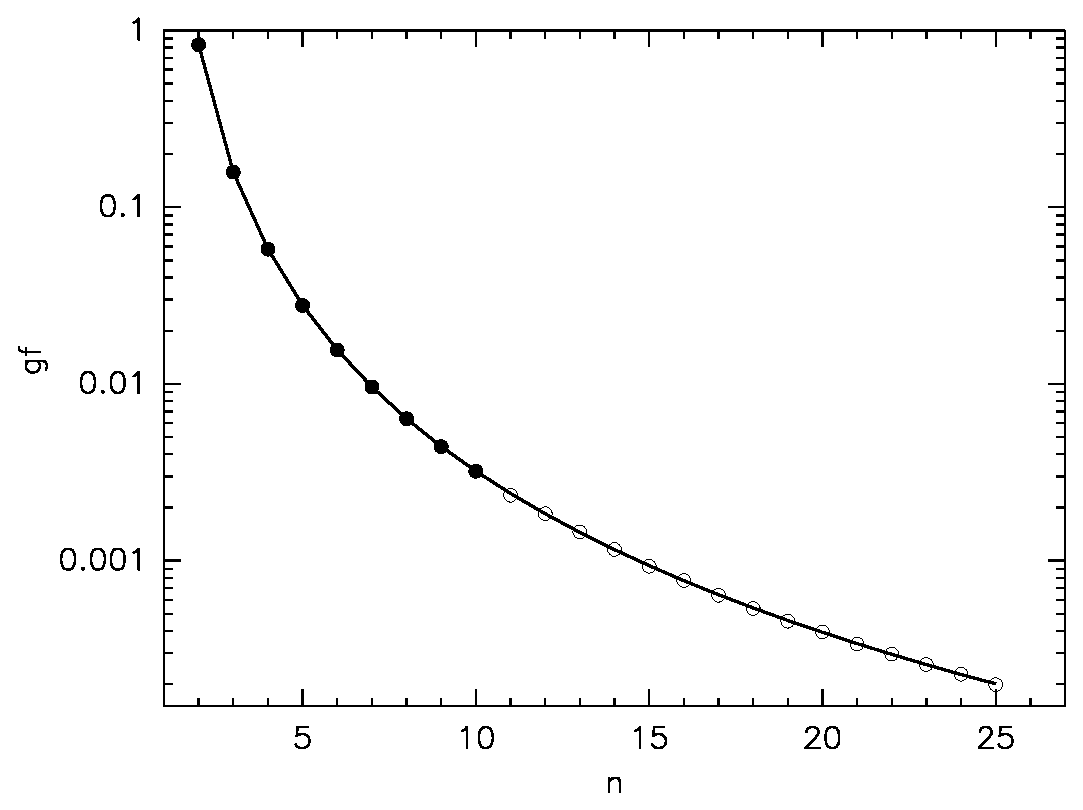
\includegraphics[width=5in]{tr.eps}
\end{figure}

\section{Conclusions}
\label{sec_conclusions}
We have developed a complete software package for calculating atomic radiative
and collisional processes. The atomic structure part of the package is
presented. Comparison of transition energies and oscillator strengths for
various ions with the results of existing codes and experimental
values shows good agreement. The program should be useful in rapidly providing
large amount of atomic data for spectral modeling.

\begin{acknowledgments}
The author would like to thank Masao Sako for his continuous test of the code
and Ehud Behar, Peter Beiersdorfer, and Mau Chen for their helpful
suggestions. The author also thanks D.H. Bailey 
of NASA Ames Research Center for his multi-precision floating point arithmetic
package included in this software. This work is supported by
NASA through Chandra Postdoctoral Fellowship Award Number PF01-10014 issued by
the Chandra X-ray Observatory Center, which is operated by Smithsonian
Astrophysical Observatory for and on behalf of NASA under contract NAS8-39073.
\end{acknowledgments}

\bibliographystyle{apsrev}
\bibliography{facref}

\end{document}
